\que{Функционал. Класс допустимых функций. Функционал в простейшей задаче
вариационного исчисления. Операции сложения функций и умножения функции на число
в классе допустимых функций. Пространство $ D_1[a, b] $.} 
\paragraph{Функционал.}
\begin{definition}
\emph{Функционалом}
называется любое отображение из некоторого класса функций ($ C^m[a, b] $, $
\mathscr R[a,b] $, \ldots) в числа
($ \mathbb R $, $ \mathbb C $, \ldots). 
\end{definition}

\textsc{Примеры.}
\begin{enumerate}
  \item Значение функции в фиксированной точке $ J_{x_0}[f] = f(x_0) $
    является функционалом, определённым на действительнозначных функциях.
  \item\label{enum1:2} Интеграл $ J_{[a,b]}[f] = \int_{a}^{b} f(x)\,dx $ является
    функционалом, определённым на пространстве $ \mathscr{R}[a,b] $
    интегрируемых на отрезке $ [a,b] $ действительнозначных функций.
  \item Более общий пример. Пусть $ F\colon \mathbb R^3 \to \mathbb R $ ---
    произвольная функция трёх переменных $ F(x, y, z) $. Подставляя вместо $ y $
    произвольную функцию $ f \in D_1[a, b] $ (так у нас обозначаются непрерывно
    дифференцируемые функции) и вместо $ z $ её производную $ f'
    $, получаем функционал  
    \[
      J[f] = \int\limits_{a}^{b}F(x, f(x), f'(x))\,dx.
    \]
   Такие функционалы в основном и рассматриваются. 
\end{enumerate}

\begin{wrapfigure}{l}{0.5\textwidth}
  \centering
  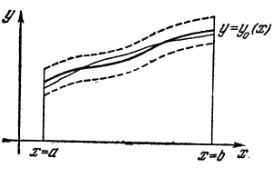
\includegraphics[width=0.4\textwidth]{Figures/norm_0.png}
  \caption{$ \varepsilon $-окрестность функции $ f $ по метрике, порождённой
  нормой $ \|\ \|_0 $.}
  \label{fig:norm_0}
\end{wrapfigure}
\paragraph{Класс допустимых функций.} Как уже было видно выше, для каждого
функционала необходимо задавать область определения --- \emph{класс допустимых
функций}. Причём если для вещественнозначных функций $ n $ переменных область
определения всегда можно было считать $ n $-мерным евклидовым пространством, то
классы допустимых функций могут существенным образом отличаться. Их определение
часто вытекает из поставленной задачи --- для примера \ref{enum1:2} логично
потребовать, чтобы классом допустимых функций были интегрируемые на отрезке
функции (что мы и сделали) и так далее.

Мало определить множество определения, на этом множестве хорошо бы определить
норму. 
Поскольку все операции (сложение и умножение на число) над функциями сохраняют
непрерывность и дифференцируемость своих аргументов (так как $ \lim[f + g] =
\lim f + \lim g $ и $ \lim \lambda f = \lambda \lim f $), то множества $ C[a,b]
$, $ D_1[a,b] $ (ровно как и $ D_k[a,b] $) являются линейными пространствами.
Стандратные нормы в вариационном исчислении --- это $ \|f\|_0 =
\max\limits_{x\in[a,b]}|f(x)| $ для
$ f(x) \in C[a,b]$ и $ \|f\|_1 = \max\limits_{x\in[a,b]}|f(x)| +
\max\limits_{x\in[a,b]}|f'(x)| $ для $ D_1[a,b] $. Таким образом, две функции $ f, g \in C[a,b] $  отличаются по норме
$ \|\ \|_0 $ менее, чем на $ \varepsilon $, если график функции $ g(x) $ целиком
лежит внутри полосы, окружающей график функции $ f(x) $ (см. рис. \ref{fig:norm_0}).
Норма $ \|\ \|_1 $ требует выполнения этого условия также для графиков $ g'(x)$,
$f'(x) $ (хотя этого и не будет достаточно).



\paragraph{Функционал в простейшей задаче вариационного
исчисления.} \emph{Простейшая задача вариационного исчисления} формулируется
так. Пусть $ F(x, y, z) $ --- функция, имеющая непрерывные частные производные
до второй включительно. Среди всех функций $ y(x) $, имеющих непрерывную
производную и удовлятворяющих условию  
\[
    y(a) = A, \quad y(b) = B,
\]
найти ту, которая доставляет слабый экстремум функционалу  
\begin{equation}\label{eq:func}
  J[y] = \int\limits_{a}^{b}F(x, y, y')\,dx.
\end{equation}
Иначе говоря, простейшая задача вариационного исчисления состоит
в отыскании слабого экстремума функционала указанного вида на множестве
всех гладких кривых, соединяющих две заданные точки.

Функционал \eqref{eq:func} может принимать значения 
\begin{itemize}[label=--]
  \item длины кривой, если  
  \[
    F(x, y, z) = \sqrt{1 + y'^2},
  \]
\item времени, за которое материальная точка под действием силы тяжести
  скатывается по заданному пути $ y $ (\emph{брахистохроны}),
\item площади фигуры, ограниченной заданной замкнутой кривой $ y $
  (\emph{изопериметрическая задача}).
\end{enumerate}

Такие функционалы, как \eqref{eq:func}, обладают так называемым свойством
<<локальности>>, которое состоит в следующем. Если мы разобьем кривую
$y = y(x)$ на части и вычислим значение функционала для каждой
из этих частей, то сумма этих значений будет равна значению
функционала для всей кривой $y = y(x)$.



\que{Нормированное пространство, нормы $ \|\ \|_0 $ и $ \|\ \|_1 $ в
пространстве $ D_1[a,b] $.}
\begin{definition*}
  \emph{Нормой} называется неотрицательная вещественнозначная функция,
  определённая на векторном пространстве $ V $, и обладающая свойствами
  \begin{enumerate}[label=\alph*)]
    \item $ \|v\| = 0 \Rightarrow v = 0 $,
    \item $ \|\lambda v\| = |\lambda| \cdot \|v\| $ (\textsc{однородность}),
    \item $ \|u + v\| \leqslant \|u\| + \|v\| $ (\textsc{неравенство
      треугольника})
  \end{enumerate}
 для любых $ u, v \in V $.

Векторное пространство с определённой нормой называют \emph{нормированным}. 
\end{definition*}


Поскольку все операции (сложение и умножение на число) над функциями сохраняют
непрерывность и дифференцируемость своих аргументов (так как $ \lim[f + g] =
\lim f + \lim g $ и $ \lim \lambda f = \lambda \lim f $), то множества $ C[a,b]
$, $ D_1[a,b] $ (ровно как и $ D_k[a,b] $) являются линейными пространствами.
Стандратные нормы в вариационном исчислении --- это $ \|f\|_0 =
\max\limits_{x\in[a,b]}|f(x)| $ для
$ f(x) \in C[a,b]$ и $ \|f\|_1 = \max\limits_{x\in[a,b]}|f(x)| +
\max\limits_{x\in[a,b]}|f'(x)| $ для $ D_1[a,b] $. Таким образом, две функции $ f, g \in C[a,b] $  отличаются по норме
$ \|\ \|_0 $ менее, чем на $ \varepsilon $, если график функции $ g(x) $ целиком
лежит внутри полосы, окружающей график функции $ f(x) $ (см. рис. \ref{fig:norm_0}).
Норма $ \|\ \|_1 $ требует выполнения этого условия также для графиков $ g'(x)$,
$f'(x) $ (хотя этого и не будет достаточно).



Проверим, что указанные функции $ \|\ \|_0 $, $ \|\ \|_1 $ действительно
являются нормами. Свойства a), b) и свойство c) для нормы $ \|\ \|_0 $ очевидно выполняются. Проверим свойство c) для
нормы $ \|\ \|_1 $. Действительно, условие
\begin{multline*}
  \| f+ g\| = \max_{x\in[a,b]}|f(x) + g(x)| + \max_{x\in[a,b]}|f'(x) + g'(x)|
  \leqslant \\ \leqslant 
  \max_{x\in[a,b]}|f(x)| + \max_{x\in[a,b]}|g(x)| +
  \max_{x\in[a,b]}|f'(x)| + \max_{x\in[a,b]}|g'(x)|
\end{multline*}
выполняется даже в случаях, когда $ \argmax f(x) = \argmax g(x) $ и $ \argmax f'(x) = \argmax
g'(x) $. В остальных же случаях всё ещё лучше.



\que{Метрическое пространство, метрики $ \rho_0 $ и $ \rho_1 $ в пространстве $
D_1[a, b]$.}
\begin{definition*}
  \emph{Метрикой} называется неотрицательная вещественнозначная функция двух
  аргументов $ \rho(x, y)\colon A \to \mathbb R$,
  определённая на произвольном множестве $ A $, со свойствами
  \begin{enumerate}[label=\alph*)]
    \item $ \rho(x, y) = 0 \Leftrightarrow x = y $,
    \item $ \rho(x, y) = \rho(y,x) $ (\textsc{симметричность}),
    \item $ \rho(x, z) \leqslant \rho(x, y) + \rho(y,z) $ (\textsc{неравенство
      треугольника})
  \end{enumerate}
  для любых $ x,y,z\in A $.

  Множество с введённой метрикой называют \emph{метрическим пространством}.
\end{definition*}


Любой нормой в векторном пространстве $ V $ индуцируется \emph{метрика} по
формуле $ \rho(x, y) = \|x - y\| $. Легко проверяется, что все свойства метрики
при этом будут выполнены.


Таким образом, в пространствах $ C[a,b] $ и $ D_1[a,b] $ индуцированная метрика
будет задаваться функциями  
\begin{align*}
  \rho_0(f, g) &= \|g - f\|_0 = \max_{x\in[a,b]}|g(x)-f(x)|,\\
  \rho_1(f, g) &= \|g - f \|_1 = \max_{x\in[a,b]}|g(x)-f(x)| +
  \max_{x\in[a,b]}|g'(x)-f'(x)|.
\end{align*}




\que{Метрики $ \rho_0 $ и $ \rho_1 $ в пространстве $ D_1[a, b] $. Окрестности
  точки в пространстве $ D_1[a,b] $
в смысле метрик $ \rho_0 $ и $ \rho_1 $, их связь.}
\begin{definition*}
  \emph{Метрикой} называется неотрицательная вещественнозначная функция двух
  аргументов $ \rho(x, y)\colon A \to \mathbb R$,
  определённая на произвольном множестве $ A $, со свойствами
  \begin{enumerate}[label=\alph*)]
    \item $ \rho(x, y) = 0 \Leftrightarrow x = y $,
    \item $ \rho(x, y) = \rho(y,x) $ (\textsc{симметричность}),
    \item $ \rho(x, z) \leqslant \rho(x, y) + \rho(y,z) $ (\textsc{неравенство
      треугольника})
  \end{enumerate}
  для любых $ x,y,z\in A $.

  Множество с введённой метрикой называют \emph{метрическим пространством}.
\end{definition*}


Любой нормой в векторном пространстве $ V $ индуцируется \emph{метрика} по
формуле $ \rho(x, y) = \|x - y\| $. Легко проверяется, что все свойства метрики
при этом будут выполнены.


Таким образом, в пространствах $ C[a,b] $ и $ D_1[a,b] $ индуцированная метрика
будет задаваться функциями  
\begin{align*}
  \rho_0(f, g) &= \|g - f\|_0 = \max_{x\in[a,b]}|g(x)-f(x)|,\\
  \rho_1(f, g) &= \|g - f \|_1 = \max_{x\in[a,b]}|g(x)-f(x)| +
  \max_{x\in[a,b]}|g'(x)-f'(x)|.
\end{align*}



\begin{definition}
  \emph{Открытым шаром} радиуса $ \varepsilon > 0 $ и центром в точке $ x_0 $ в метрическом пространстве $ A $ называется
  множество точек, удовлетворящих условию $ \rho(x_0, x) < \varepsilon $.
\end{definition}
\begin{definition}
  \emph{Открытым множеством} в метрическом пространстве $ A $ называется множество
 точек $ U $, каждая из которых содержится в $ U $ вместе с некоторым шаром с центром в
 этой точке.
\end{definition}
\begin{definition}
  \emph{Окрестностью} точки $ x_0 $ называется любое открытое множество,
  содержащее эту точку (в русской традиции).
\end{definition}

Таким образом, на рисунке \ref{fig:norm_0} изображена \emph{$ \varepsilon
$-окрестность} точки (функции) $ f $ --- шар с центром в $ f $ и радиусом $
\varepsilon $, а функция $ g $ в том же примере принадлежит
$ \varepsilon $-окрестности $ f $.

Окрестность в смысле метрики $ \rho_1 $ ставит дополнительное ограничение на рост функции.
При этом чем больше отличаются функции $ f $, $ g $ в смысле метрики $ \rho_0 $,
тем меньше они должны отличаться своим ростом в точках.

Понятно что любая окрестность в смысле $ C_1 $ будет окрестностью в смысле $ D_1
$, но не наоборот.


\que{Нормированное пространство. Метрическое пространство.
Связь между этими понятиями.}
\begin{definition*}
  \emph{Нормой} называется неотрицательная вещественнозначная функция,
  определённая на векторном пространстве $ V $, и обладающая свойствами
  \begin{enumerate}[label=\alph*)]
    \item $ \|v\| = 0 \Rightarrow v = 0 $,
    \item $ \|\lambda v\| = |\lambda| \cdot \|v\| $ (\textsc{однородность}),
    \item $ \|u + v\| \leqslant \|u\| + \|v\| $ (\textsc{неравенство
      треугольника})
  \end{enumerate}
 для любых $ u, v \in V $.

Векторное пространство с определённой нормой называют \emph{нормированным}. 
\end{definition*}


\begin{definition*}
  \emph{Метрикой} называется неотрицательная вещественнозначная функция двух
  аргументов $ \rho(x, y)\colon A \to \mathbb R$,
  определённая на произвольном множестве $ A $, со свойствами
  \begin{enumerate}[label=\alph*)]
    \item $ \rho(x, y) = 0 \Leftrightarrow x = y $,
    \item $ \rho(x, y) = \rho(y,x) $ (\textsc{симметричность}),
    \item $ \rho(x, z) \leqslant \rho(x, y) + \rho(y,z) $ (\textsc{неравенство
      треугольника})
  \end{enumerate}
  для любых $ x,y,z\in A $.

  Множество с введённой метрикой называют \emph{метрическим пространством}.
\end{definition*}



Однако одной метрики, вообще говоря, не хватит, чтобы ввести норму. Во-первых,
метрика задаётся на произвольном множестве, а норма может быть определена только
на линейном пространстве. Но даже введённая на линейном пространстве метрика
может не оказаться нормой в смысле $ \|x\| = \rho(0, x) $ из-за условия
однородности b) для нормы.
